\clearpage
\section{Analyse}
\subsection{Vergleich der Algorithmen}
Bei den Experimenten mit den verschiedenen Algorithmen ist aufgefallen, dass der Emoticon Algorithmus aufgrund der seltenen Verwendung von Emoticons in Tweets praktisch nicht funktioniert. Je ernster das Thema desto weniger Emoticons werden tendenziell verwendet. Folgend die Resultate zweier Twitter Downloads. Die Keywörter für den ersten Download waren \flqq switzerland \frqq und \flqq ecuador\frqq. Die Schweiz hat kurz zuvor am WM Auftaktspiel in der 93. Minute das entscheidende 2:1 gegen Ecuador geschossen. Die Keywörter für den zweiten Download waren \flqq ISIS\frqq und \flqq Iraq\flqq. ISIS ist eine militante Jihadistengruppe, die derzeit für unruhen im Nordiran sorgt. \cite{isis} Folgend werden diese Resultate beschrieben und es werden Thesen zu den Resultaten der Twitteranalysen aufgestellt. Um diese zu verifizieren oder zu falsifizieren, bräuchte man gelabelte Twitterdaten, welche im Rahmen dieser Arbeit nicht erarbeitet werden konnten.

\begin{figure}[h]
  \centering
  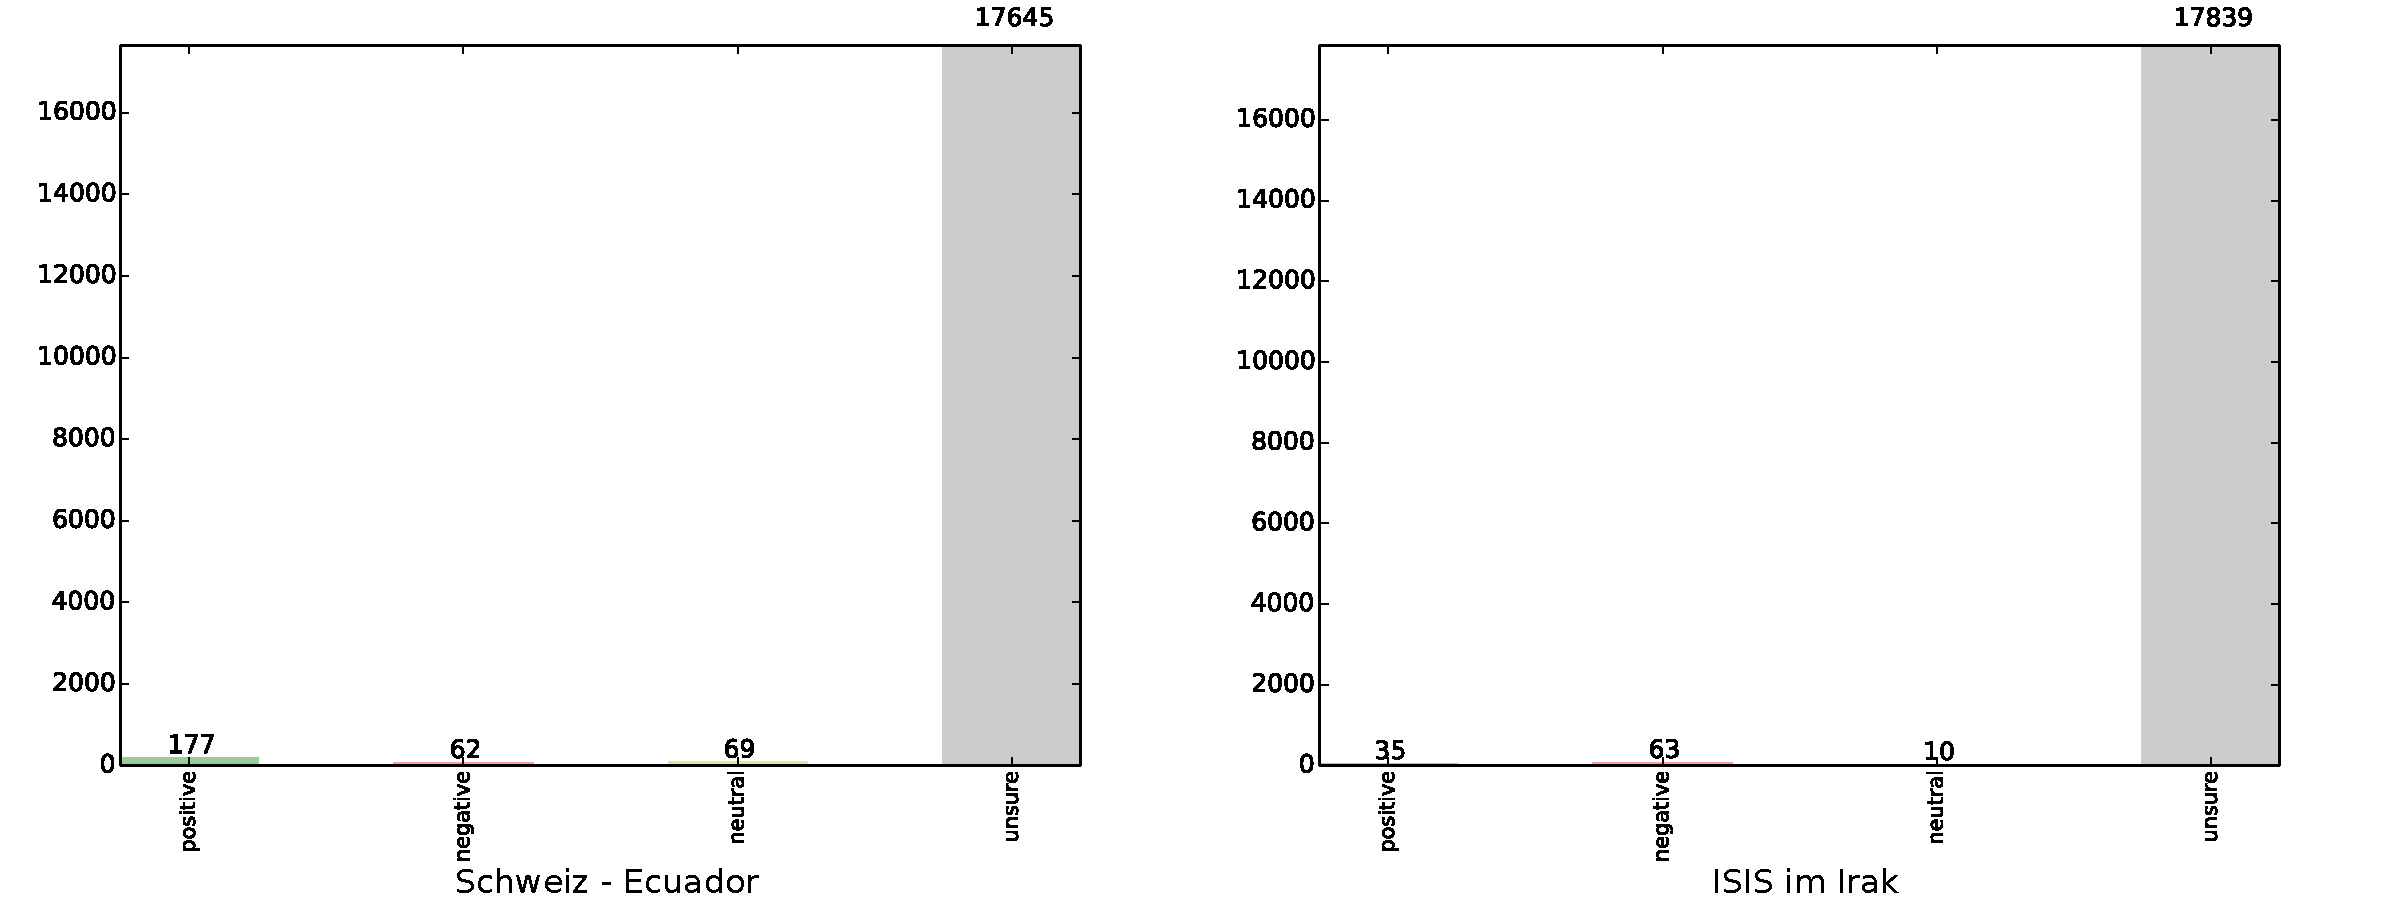
\includegraphics[width=0.8\textwidth]{images/schweizvsirak_emoticon.pdf}
  \caption[Emoticon Analyse: Schweiz - Ecuador vs. ISIS im Irak]{Emoticon Analyse: Schweiz - Ecuador vs. ISIS im Irak}
  \label{fig:emoticonanalysis}
\end{figure}

Die Resultate der in Abbildung \ref{fig:emoticonanalysis} sichtbaren Suche decken sich mit den Erkenntnissen aus vorhergehenden Suchläufen. In rund 1.7\% der Schweiz-Ecuador Tweets wurden Emoticons verwendet. Erfreulicherweise waren diese mehrheitlich positiv. Die Irak Tweets hatten lediglich einen Emoticon-Anteil von 0.6\% und diese waren meist negativ.

Beim der Twitteranalyse mithilfe des naiven Bayes der NLTK Library (Abbildung \ref{fig:naivebayesanalysis}) ist ersichtlich, wie sich die Wahl des Trainingsets auf das Ergebnis auswirkt. Movie Reviews (das hier verwendete Trainingset) sind üblicherweise längere Texte die, wenn positiv, sehr sachlich geschrieben sind. Beim manuellen durchsehen der Tweets fiel auf, dass viele Tweets zu ISIS im Irak Zeitungsüberschriften entsprechen oder einfach sehr sachlich geschrieben sind. Dies wird von diesem Klassifizierungsverfahren als positiv gewertet.

\begin{figure}[H]
  \centering
  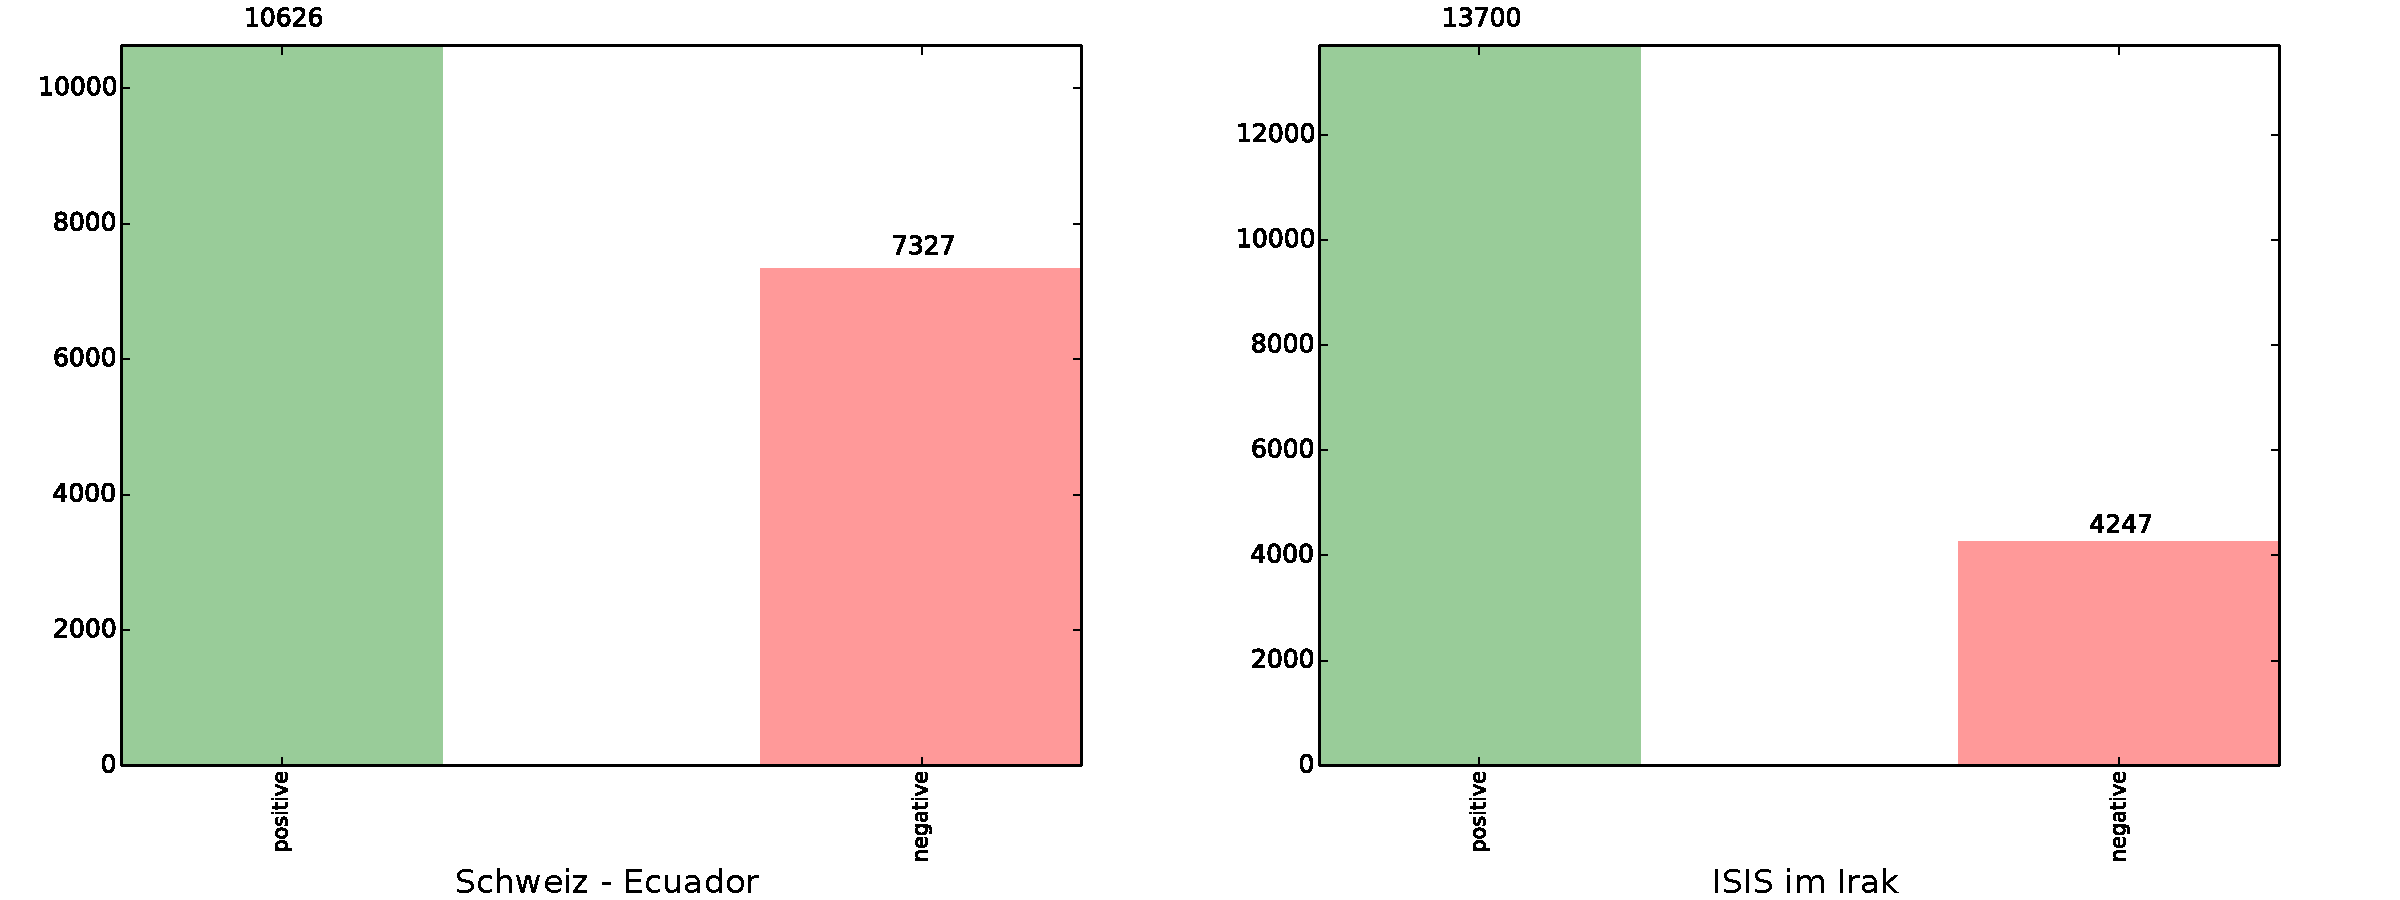
\includegraphics[width=0.8\textwidth]{images/schweizvsirak_nltk.pdf}
  \caption[NLTK Naive Bayes: Schweiz - Ecuador vs. ISIS im Irak]{NLTK Naive Bayes: Schweiz - Ecuador vs. ISIS im Irak}
  \label{fig:naivebayesanalysis}
\end{figure}

\begin{figure}[H]
  \centering
  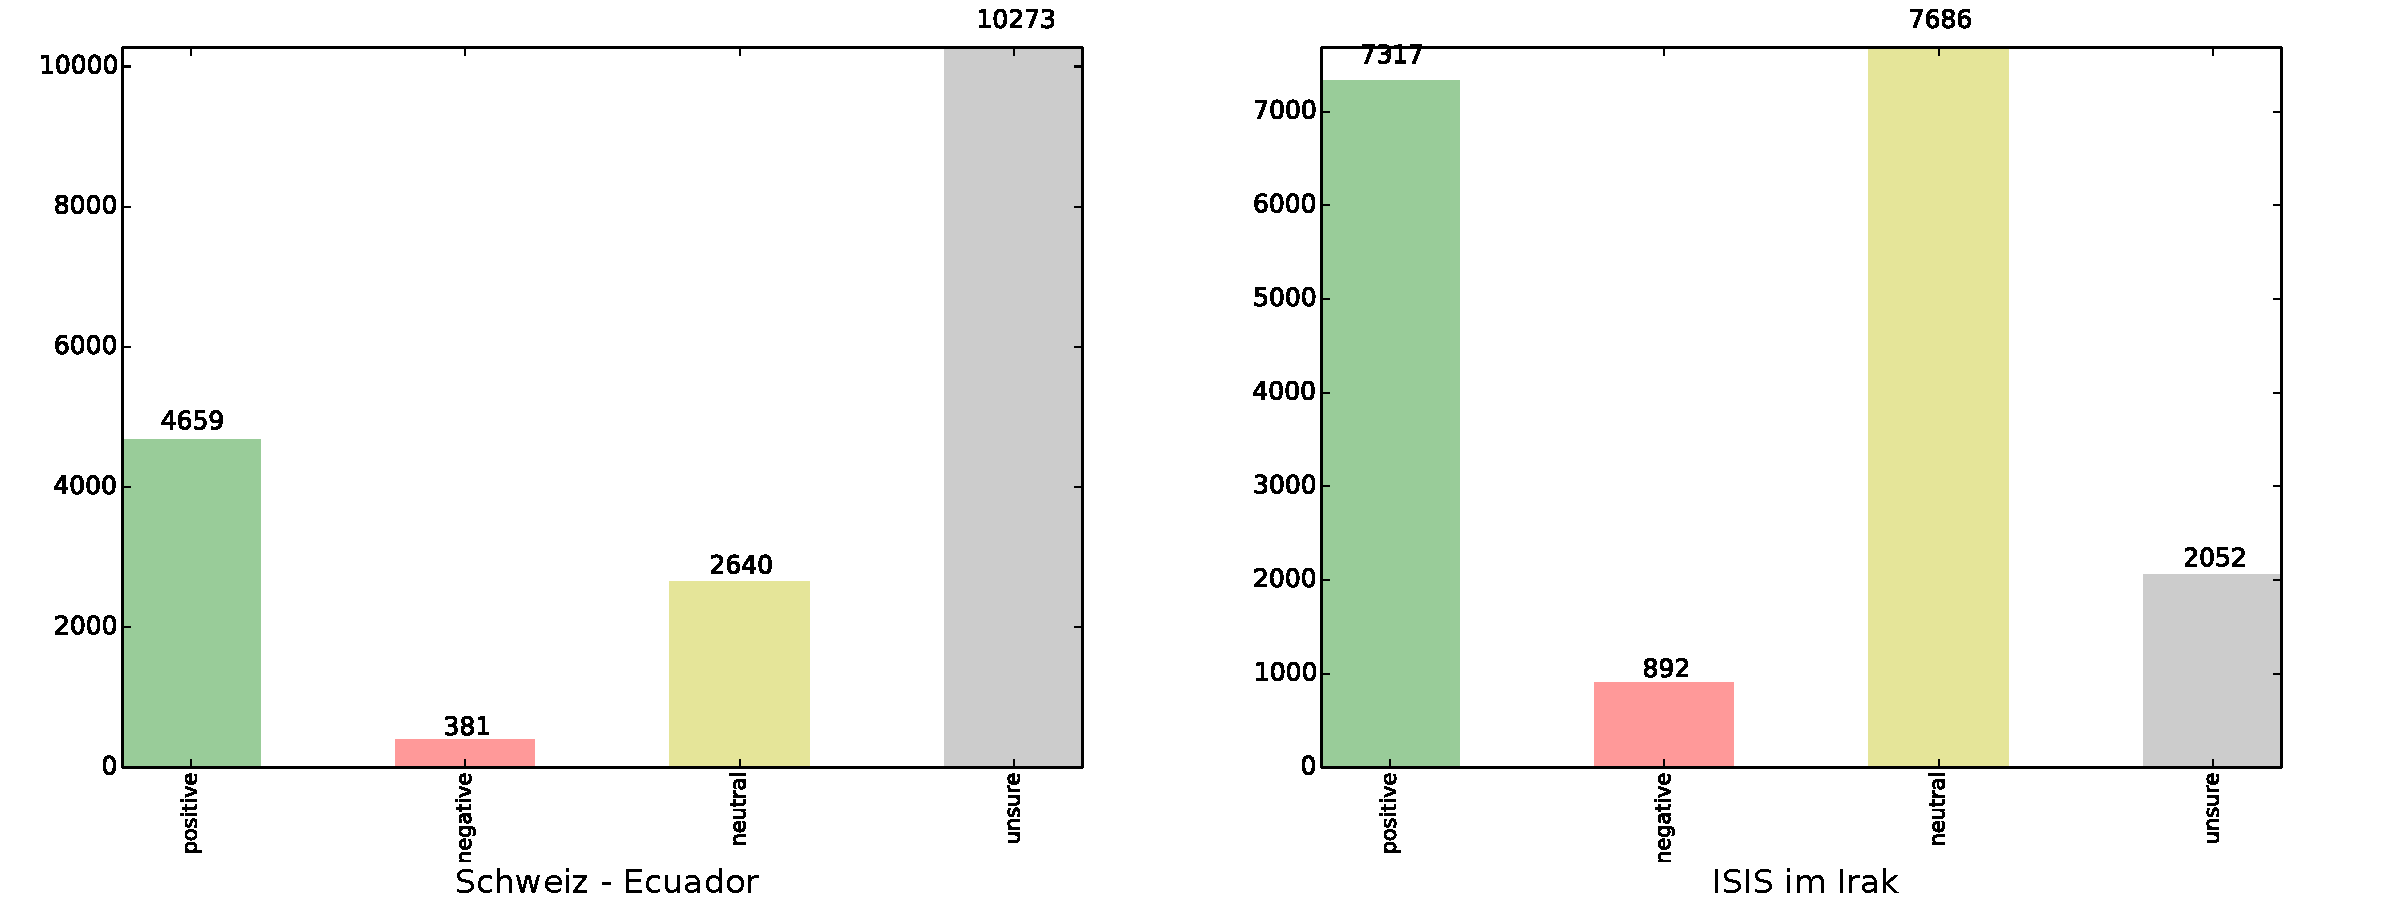
\includegraphics[width=0.8\textwidth]{images/schweizvsirak_sasa.pdf}
  \caption[SASA: Schweiz - Ecuador vs. ISIS im Irak]{SASA: Schweiz - Ecuador vs. ISIS im Irak}
  \label{fig:sasaanalysis}
\end{figure}

\begin{figure}[H]
  \centering
  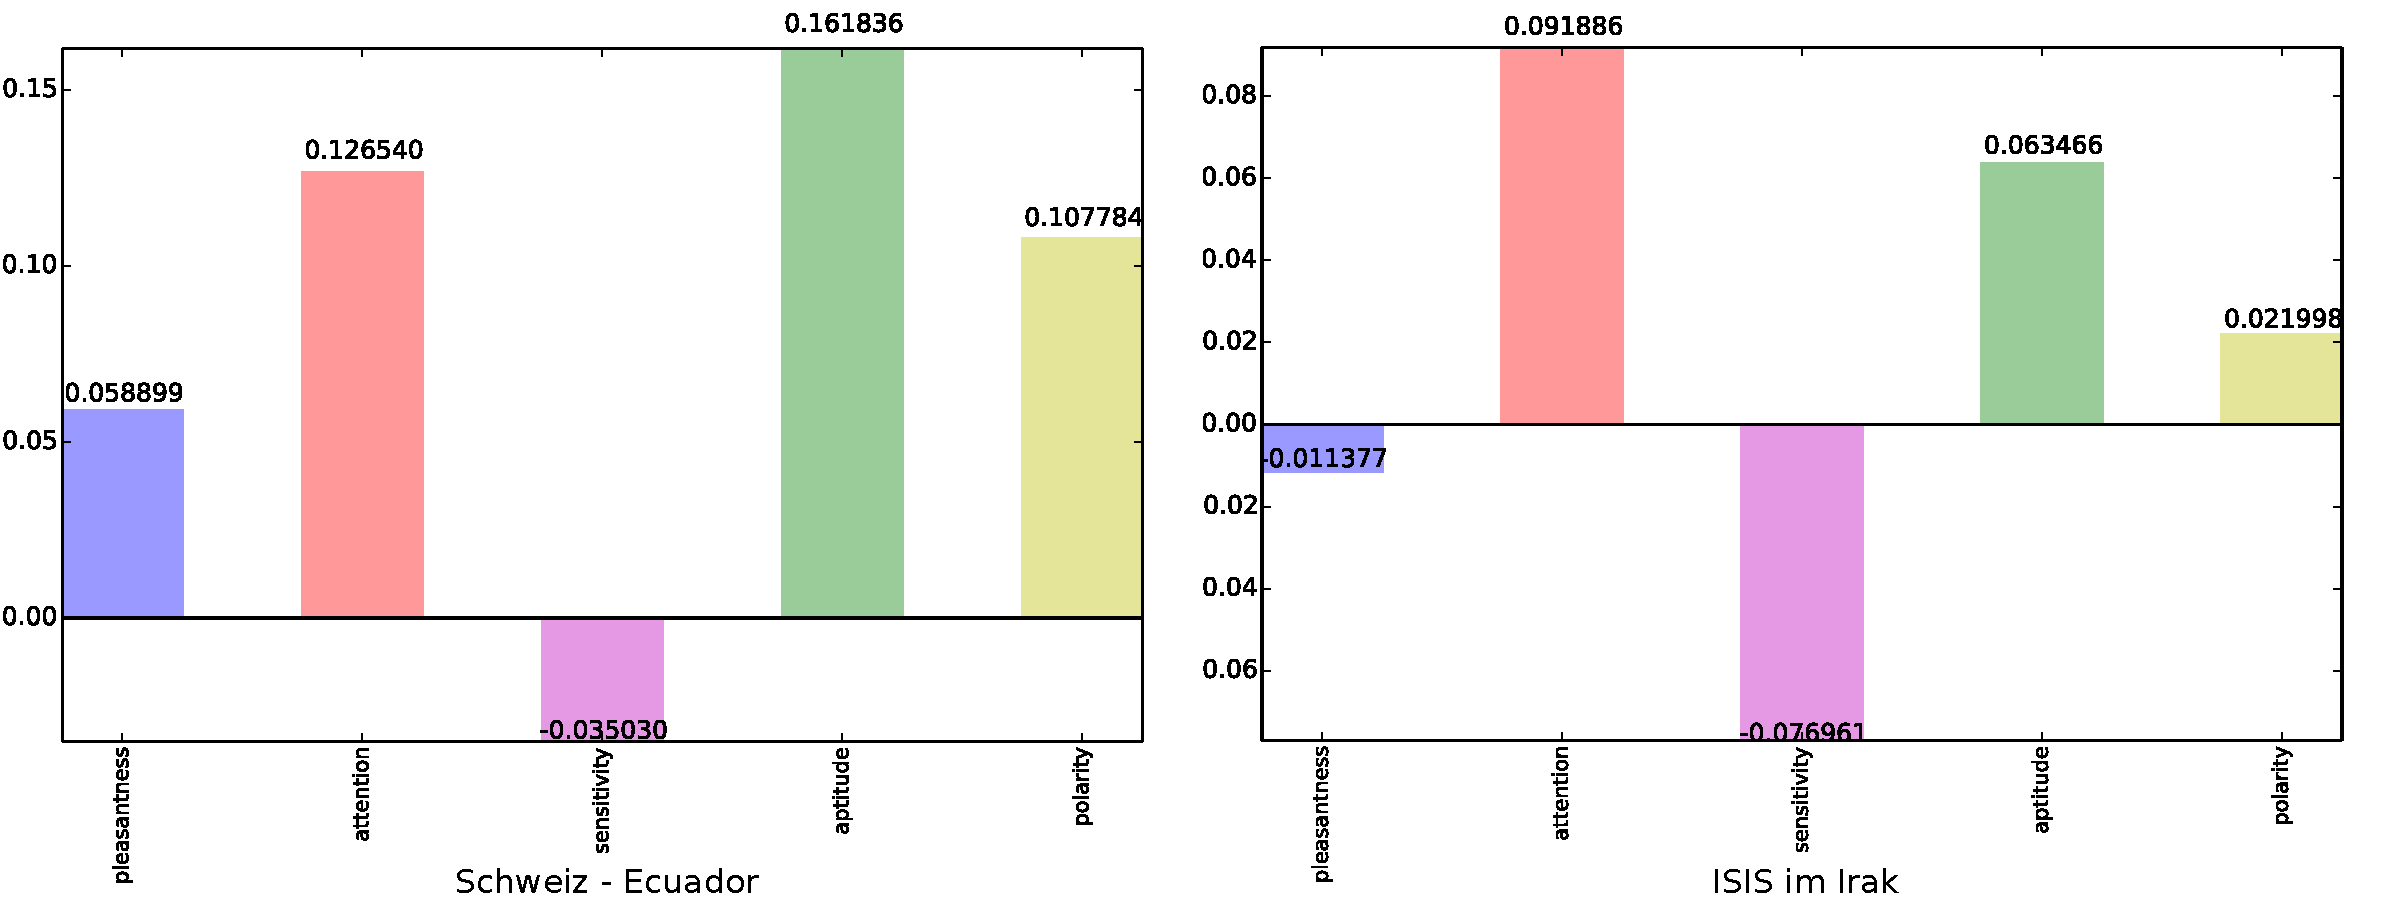
\includegraphics[width=0.8\textwidth]{images/schweizvsirak_senticnet.pdf}
  \caption[SenticNet: Schweiz - Ecuador vs. ISIS im Irak]{SASA: Schweiz - Ecuador vs. ISIS im Irak}
  \label{fig:senticnetanalysis}
\end{figure}

Die SASA Library (vgl. Abbildung \ref{fig:sasaanalysis}) hat viele der Irak-Tweets als neutral gelabelt. Dies würde sich mit meiner Beobachtung der vielen Zeitungsüberschriften decken. Weiter scheint der Algorithmus Probleme mit den sehr kurzen Tweets im Stil von \flqq \#Switzerland beats \#ecuador 2-1 at World \#EnnerValencia \#WorldCups\frqq zu haben. Er Kategorisiert diese gar nicht erst. 

Der SenticNet (vgl. Abbildung \ref{fig:senticnetanalysis}) Algorithmus zeigt für die Schweiz-Ecuador Tweets deutlich positivere Resultate als für die Tweets zum Treiben der ISIS Jihadisten im Irak. Diese Resultate scheinen plausibel zu sein.

\begin{figure}[h]
  \centering
  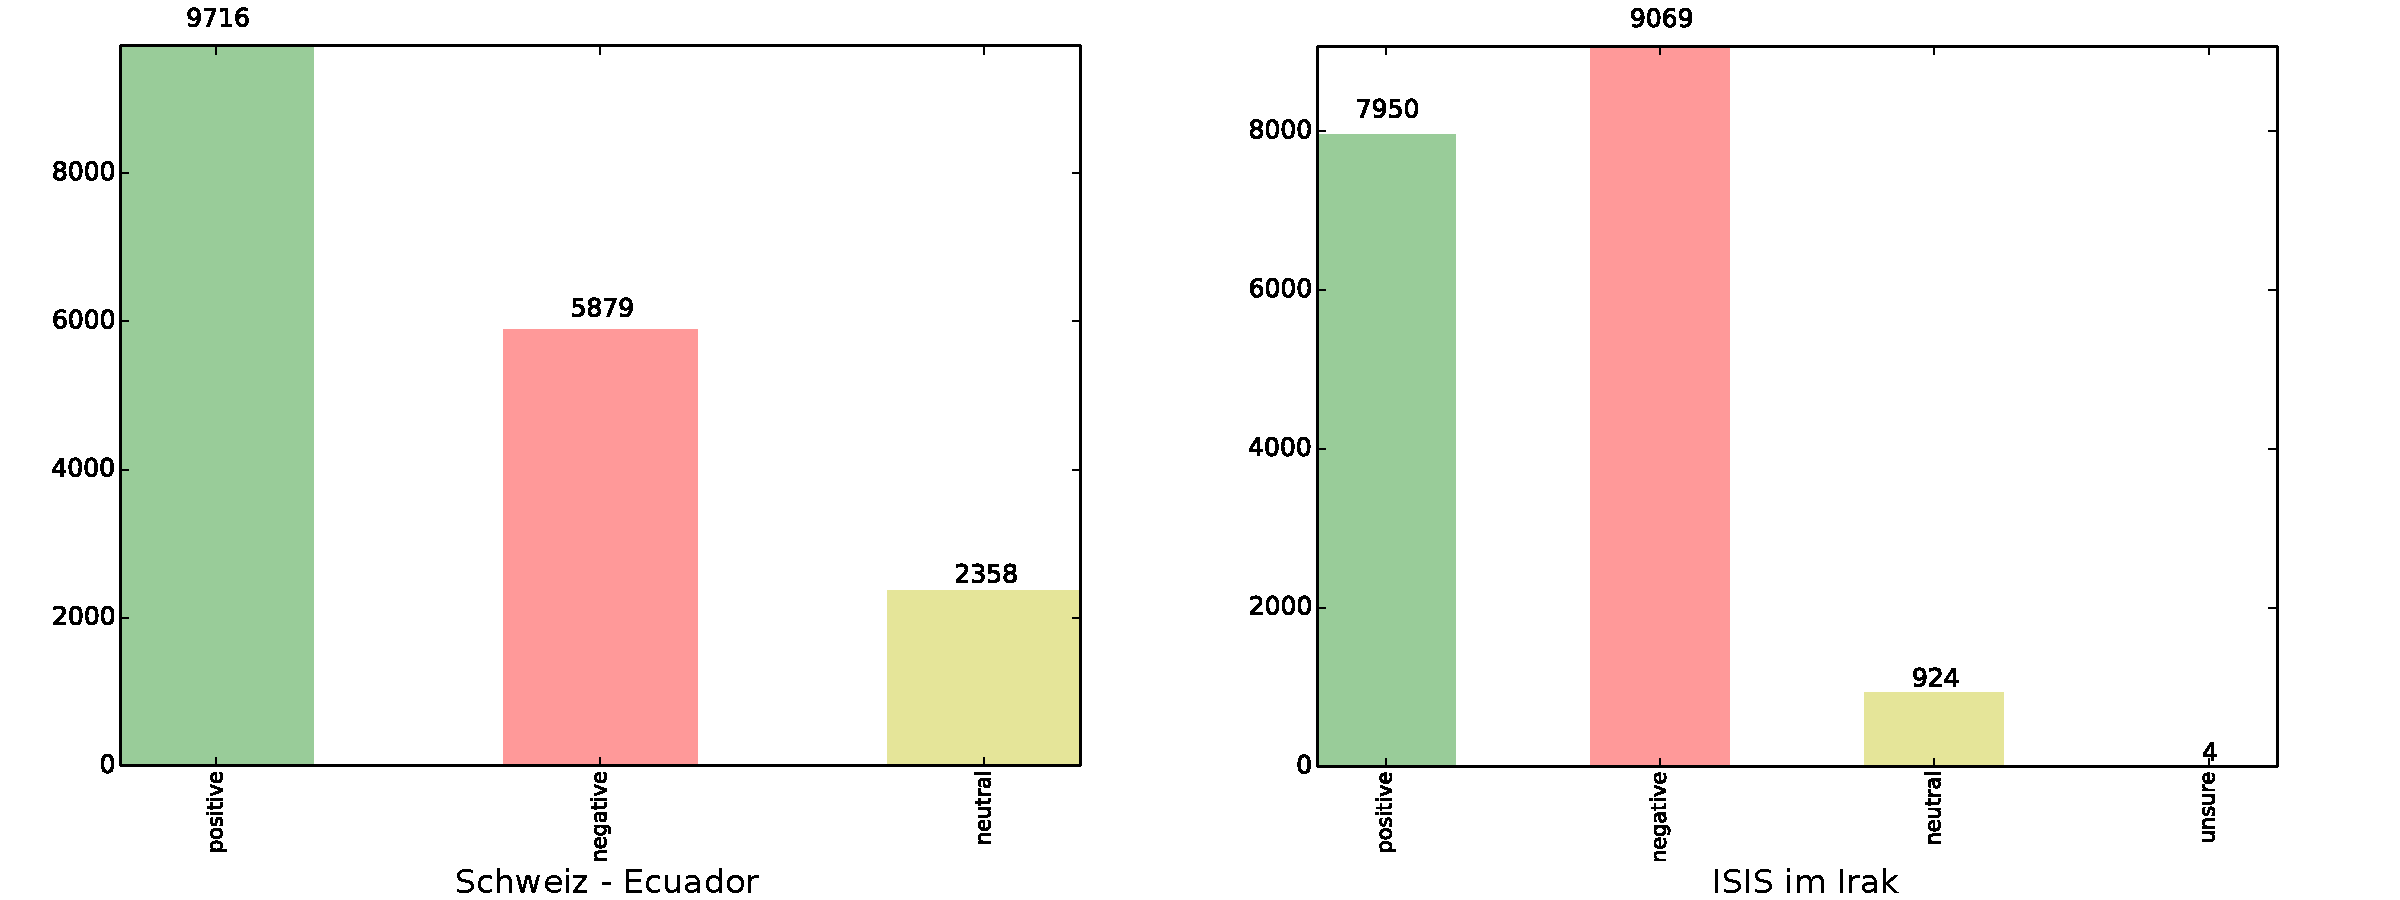
\includegraphics[width=0.8\textwidth]{images/schweizvsirak_sentiwordnet.pdf}
  \caption[SentiWordNet: Schweiz - Ecuador vs. ISIS im Irak]{SentiWordNet: Schweiz - Ecuador vs. ISIS im Irak}
  \label{fig:sentiwordnet}
\end{figure}

Auch die Resultate des SentiWordNet (Abbildung \ref{fig:sentiwordnet}) scheinen plausibel zu sein. Hier werden negative Emotionen aus den ISIS Tweets herausgelesen und das Schweizer Tor in der 93. Minuten wird zwar von der Mehrheit, jedoch nicht von allen Twitterern positiv beschrieben.

Diese Beobachtungen decken sich mit den Erkenntnissen von Pollyanna Gonçalves et al. \cite{comparing}. Um wirklich etwas darüber auszusagen müsste gefilterte, bereinigte und manuell klassifizierte Tweets zu unterschiedlichen Themen untersuchen.

\clearpage
\subsection{Parallelisierung}
Die Vorteile der Parallelisierung auf meinem 4-Kerne System waren bereits ab wenigen tausend Tweets spürbar. Um zu sehen wie viel die Parallelisierung wirklich aus macht, wurden die Tweets über die ISIS Jihadisten mehrfach mit unterschiedlicher Anzahl Prozesse vom Programm analysiert. Dabei sind mir vor allem Unterschiede in den Zeiten für die Analysen an sich (der parallelisierte Teil) und der Initialisierung ins Auge gefallen. 

\begin{figure}[h]
  \centering
  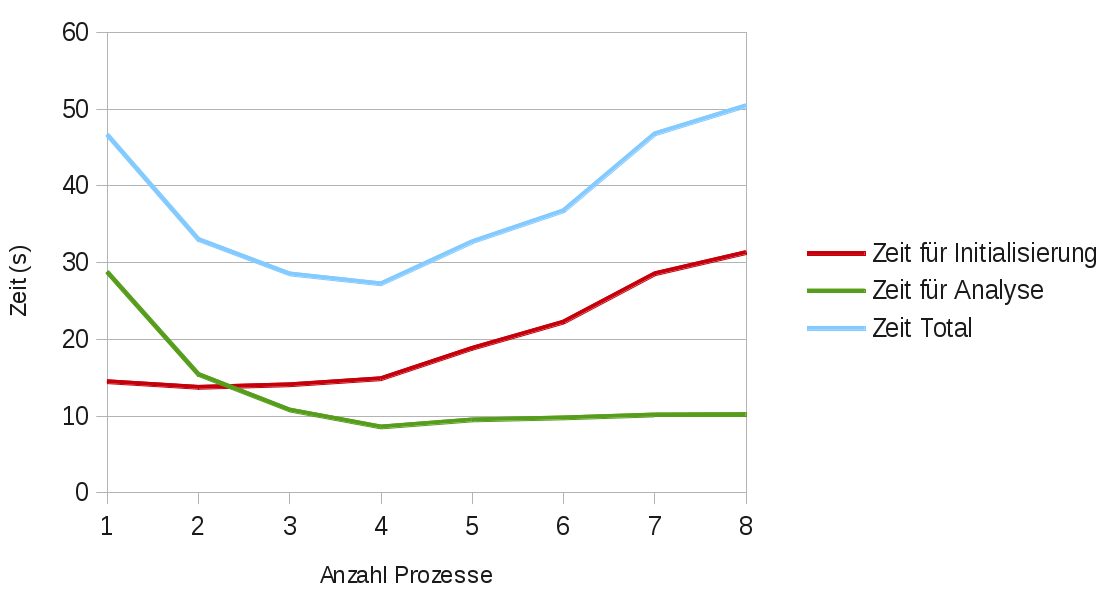
\includegraphics[width=0.8\textwidth]{images/parallelisierung_chart.png}
  \caption[Laufzeitverhalten bei unterschiedlicher Anzahl Prozesse]{Laufzeitverhalten bei unterschiedlicher Anzahl Prozesse}
  \label{fig:analyseparallel}
\end{figure}


In der Abbildung \ref{fig:analyseparallel} ist ersichtlich, wie die Zeit für die Initialisierung bis zum erreichen der physisch vorhandenen 4-Kerne praktisch konstant bleibt. Wenn man die Anzahl Prozesse weiter erhöht, nimmt die Dauer für die Initialisierung stark zu. Dies liegt daran, dass sowohl der SASA Algorithmus als auch der NLTK Classifier für jeden Prozess initialisiert werden müssen. Diese Initialisierungen sind sehr aufwändig und wenn die physisch vorhandenen 4-Kerne diese Aufgabe für mehr als 4 Prozesse erledigen sollen, dauert dies entsprechend länger.

Die Zeit für die Analyse ist bei einem Prozess am höchsten, und nimmt bis zum erreichen der 4 vorhandenen Cores um fast $\frac{2}{3}$ von 30s auf unter 10s ab. Wenn mehr Prozesse verwendet werden, wird diese Zeit nicht merklich erhöht aber sie nimmt auch nicht mehr ab.

Daraus lässt sich schlussfolgern, dass in dem gegebenen Setup 4 Prozesse die beste Performance bieten. Weiter könnte man daraus ableiten, dass die optimale Anzahl Prozesse der Anzahl verfügbarer Cores entspricht. Diese These könnte unter gleichen Testbedingungen auf verschiedenen Setups weiter untersucht und gegebenenfalls verifiziert oder falsifiziert werden. Die Einstellung zur Anzahl Prozesse kann im \lstinline$starter.py$ angepasst werden.